
\subsection{Tagging Tracker Performance (Editors: Tim Nelson, Omar Moreno)}

The tagging tracker must identify incoming beam-energy electrons with extremely high purity, suppressing the mis-reconstruction of any incoming low-momentum charged particles as beam energy electrons. In particular, any incoming charged particle within the recoil acceptance for signal that is reconstructed as having the beam energy in the tagging tracker is an irreducible background. The design of the tagging tracker makes the likelihood of such errors vanishingly small, with good resolution for both beam energy and off-energy incoming tracks and an exceedingly low rate of mis-reconstruction for tracks within the recoil energy acceptance.

In order for an incoming low momentum particle to fake a beam energy electron in the tagger, a number of conditions must simultaneously be met:
\begin{enumerate}
    \item The incoming particle must reach the first tagger layer or it will not intersect with any material until it hits the wall of the vacuum chamber.
    \item The particle must either scatter in each layer in order to fake a 4 GeV track or create secondaries that generate occupancy which confuses the pattern recognition in the tracker resulting in reconstruction of a fake 4 GeV track.
    \item The resulting track must have a trajectory consistent with that of a typical 4 GeV beam electron all the way through the tracker.
    \item The resulting track must have an impact point at the target consistent with a reconstructed track within the signal acceptance in the recoil tracker. 
\end{enumerate}
Using an analytic model of the tagging tracker that includes the effect of intrinsic resolutions and multiple scattering in the tracker planes, it is evident that each of these requirements places a very heavy penalty on any off-energy component in the beam.  First, incoming particles with less than approximately 500 MeV momentum will not hit the first layer of the tagger unless they are significantly off-trajectory as well.  Furthermore, even at 500 MeV, a first scatter of more than 10$^\circ$ is needed in order for the incoming particle to appear to be on the correct trajectory. It is clear then that the most challenging scenario is large contamination with incoming charged particles at the top of the momentum range for signal recoils, nominally 1.2 GeV.  Such particles have the highest likelihood of reaching the first layer of the tagger tracker without being bent away by the magnetic field and require much smaller scatters and/or track reconstruction errors to result in fake tags. In order for a 1.2 GeV particle to make a trajectory through the tracker consistent with a 4 GeV track, six successive scatters of approximately ten milliradians must occur, each equivalent to approximately 15$\sigma$ on the multiple scattering distribution. From the tails of the Moliere scattering distribution, the likelihood of each of these scatters is smaller than one per million.  Therefore, the much more likely scenario is the generation of secondaries an the material of the tagger tracker followed by misreconstruction of a fake 4 GeV track.  Since the resulting 4 GeV track must arrive at the target on the correct trajectory and beam energy electrons arrive normal to the target with a one-sigma error of 250 microradians, there is very little phase space for randomly reconstructed 4 GeV fakes to have the correct trajectory.  Finally, any falsely reconstructed 4 GeV track must have a common impact point in the target with a real track of matching momentum in the recoil tracker, which is unlikely for a falsely reconstructed tracks.

In order to more fully test these scenarios, two samples of incident electrons were simulated and reconstructed in the tagger tracker.  The first is a sample of XXX 4 GeV electrons on the nominal beam trajectory.  The second is a sample of XXX 1.2 GeV electrons on a trajectory that allows them to pass through all seven layers of the tagging tracker.  The 4 GeV sample confirms the expected resolutions, as shown in
Figures~\ref{fig:trackin_4gev_p}.  
%=======================
\begin{figure}[htp]
    \centering
    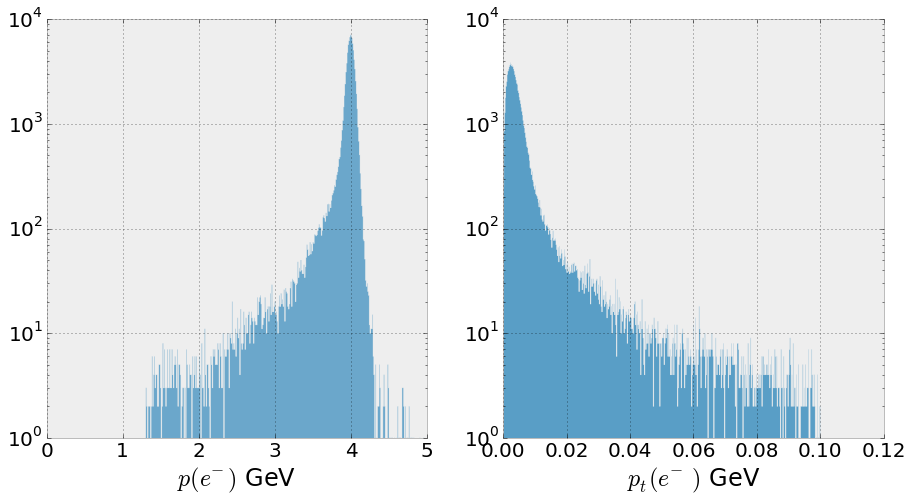
\includegraphics[width=\textwidth]{images/tagger_tracker_p_pt_4pt0_gev.png}
    \caption{\small{Reconstructed total momentum and momentum transverse to 
                    target for a sample of 4 GeV beam electrons.}}
    \label{fig:tracking_4gev_p}
\end{figure}
%=======================
%=======================
\begin{figure}[htp]
    \centering
    %    \includegraphics[width=7cm]{figures/dummy}
    \caption{\small{Reconstructed Tagger track $x$-$y$ position at the target for a
    sample of 4 GeV beam electrons.}}
    \label{fig:tracking_4gev_pos}
    %\vspace*{-5mm}
\end{figure}
%=======================

These indicate that tight requirements can be made in both the energy and trajectory at the target that rejects off-momentum particles that could be present in the incoming beam and that the tagging tracker identifies a precise impact position that can be used for tracking recoil candidates.  The 1.2 GeV sample confirms at the level of 1 part in 10$^?$ that these tracks cannot be mistaken for 4 GeV tracks, as shown in Figure~\ref{fig:tracking_1pt2gev}.  
%=======================
\begin{figure}[htp]
    \centering
    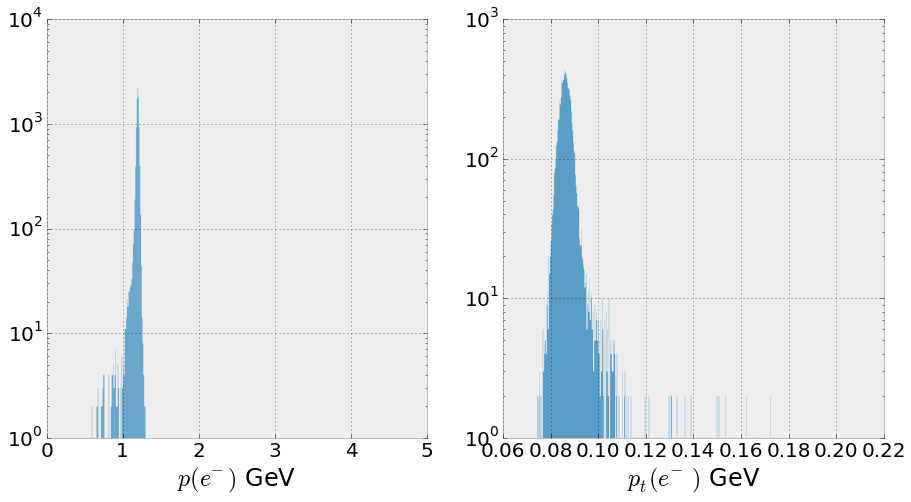
\includegraphics[width=\textwidth]{images/tagger_tracker_p_pt_1pt2_gev.png}
    \caption{\small{Reconstructed total momentum for a sample of 1.2 GeV beam 
                    electrons.}}
    \label{fig:tracking_1pt2gev}
\end{figure}
%=======================
In order to probe the likelihood of reconstructing fake 4 GeV tracks at higher statistics we further introduce random noise hits on all planes of the tracker at rates of $10^{-3}$, $10^{-2}$ and $10^{-1}$ in all planes of the tracker, where typical noise occupancies in similar HPS modules are roughy $10^{-4}$. Figure~\ref{fig:tracking_1pt2gev_noise} shows the resulting distribution of reconstructed tracks in energy and $p_T$ at the target. Obviously, such extreme occupancies in the tracker are atypical, and would easily be selected against with negligible impact on signal efficiency. 
%=======================
\begin{figure}[htp]
    \centering
    %    \includegraphics[width=7cm]{figures/dummy}
    \caption{\small{Reconstructed momentum vs. momentum transverse to the target for a sample of 1.2 GeV electrons in the presence of $10^{-3}$, $10^{-2}$ and $10^{-1}$ random occupancy in all sensors.} }
    \label{fig:tracking_1pt2gev_noise}
    %\vspace*{-5mm}
\end{figure}
%=======================
Furthermore, these fake tracks, not being due to an individual low-momentum track, will typically not align with a low-momentum track in the recoil tracker.  Although further study will be required to find the beam intensity limits for this tagging tracker design, we can safely conclude that it is more than capable of providing the tagging purity required for the first stage of the LDMX experiment.


\subsection{Recoil Tracker Performance, (Editors: Tim Nelson, Omar Moreno)}

The recoil tracker must have good efficiency for reconstructing the recoiling electrons characteristic of signal events with good resolution for transverse momentum and impact position at the target which are critical for eliminating background. In addition, the tracker should have sufficient momentum resolution that it can assist the ECal in identifying events where an incoming beam electron passes through the target and tracker without significant energy loss. Finally, the recoil tracker must help identify background events from other hard processes that can occur in the target or the tracker itself. These backgrounds include electromagnetic tridents and other events with multiple charged tracks as well as hard bremsstrahlung events where the photon undergoes a photonuclear reaction in the target or the material of the tracker.  

Estimation of the recoil momentum transverse to the target requires precise determination of the angle at the target together with a good curvature measurement to set the overall momentum scale.  At least two 3-d measurements directly downstream of the target are needed to determine the recoil angle while at least one additional bend-plane measurement is needed for curvature.  For low-momentum tracks, this third measurement can be in the first four closely-spaced layers, but for high momentum tracks that are nearly straight, hits in both of the downstream axial layers are required.  Because high-momentum signal recoils will nearly always pass through all six layers, the acceptance near the top of the energy range for signal recoils is near unity, only reduced by the single-hit efficiency in the last two layers. However, at low momentum a large number of tracks can escape detection. Therefore, in order to estimate the signal acceptance for well-measured recoils, we require that recoiling electrons leave hits in at least three of the 3-d layers, for pattern recognition and angle estimation, and at least four hits total for reasonably purity.  The tracker acceptance for signal recoils as a function of mediator mass is shown in Figure XXX.

The ability to distinguish signal from background using the recoil transverse momentum is obviously limited by the multiple scattering in the target, where multiple scattering in a 10\% $X_0$ target results in a 4 MeV smearing in transverse momentum.  Using an analytic model of the target and recoil tracker, the material budget and single-hit resolutions of the recoil tracker have been designed so that the experimental resolution is limited by multiple scattering in the target over the entire momentum range for signal recoils.










%For signal recoils with momentum greater than about 500 MeV, the six-hit acceptance for the recoil tracker is close to unity.  However, at the lowest momenta being considered for signal, 50 MeV, many  tracks will fail to hit layers 5 or 6.  In order for a
%
%
%The goal is to achieve good signal acceptance
%
%
%
%Signal recoils with momenta near the top of the 
%
%With the target range of 50 MeV to 1.2 GeV for signal recoils, 
%
%
%
%
%
%Placement of the recoil tracker in the lower fringe field of the analyzing dipole, together with the wide aspect ratio of the recoil tracker ensures good acceptance for recoils
%
%
%
%
%
%
%
%
%In order to provide good sensitivity for a broad range of dark matter and mediator masses, the goal for LDMX is acceptance of recoils having energies from approximately 50 MeV to 1.2 GeV, as much as two orders of magnitude lower than the incoming electron energy.  Meanwhile, 
%
%
%
% Additionally, the recoil tracker must have sufficient momentum resolution to aid the ECal in correctly distinguishing non-interacting beam electrons from
%
%
%
%Needs to be spelled out in more detail...
%\begin{itemize}
%    \item Acceptance
%    \item Efficiency 
%    \item What kind of activity cuts do we want to apply?  Background rejection
%        power?  Signal efficiency? 
%\end{itemize}




